\documentclass[12pt, a4paper, openany]{report}

\def\VersionRapport{1.0}

\usepackage[utf8]{inputenc} % un package
\usepackage[T1]{fontenc}      % un second package
\usepackage[francais]{babel}  % un troisième package
\usepackage{layout}
\usepackage[top=2.7cm, bottom=2.5cm, left=3.5cm, right=3cm]{geometry}
\usepackage{setspace}

\frenchbsetup{StandardLists=true} % à inclure si on utilise \usepackage[french]{babel}
%\usepackage{enumitem}
\usepackage[shortlabels]{enumitem}
\usepackage{amssymb}

\usepackage{color}
\usepackage{listings}
\definecolor{dkgreen}{rgb}{0,0.6,0}
\definecolor{gray}{rgb}{0.5,0.5,0.5}
\definecolor{mauve}{rgb}{0.58,0,0.82}
\definecolor{rougecerise}{rgb}{0.73,0.043,0.043}

\lstset{frame=tb,
  language=Matlab,
  aboveskip=3mm,
  belowskip=3mm,
  showstringspaces=false,
  columns=flexible,
  basicstyle={\small\ttfamily},
  keywordstyle=\color{blue},
  commentstyle=\color{dkgreen},
  stringstyle=\color{mauve},
  breaklines=true,
  breakatwhitespace=true,
  tabsize=3,
  breaklines=true,
  morekeywords={matlab2tikz},
  morekeywords=[2]{1}, 
  keywordstyle=[2]{\color{black}},
  identifierstyle=\color{black},
  numbers=left,
  numberstyle={\tiny \color{black}},
  numbersep=9pt, 
  emph=[1]{for,end,break},
  emphstyle=[1]\color{red}
}

\usepackage{multirow} % pour les tableaux
\usepackage[table]{xcolor} % pour les tableaux

\usepackage{verbatim}

%\usepackage{subcaption}
\usepackage{graphicx}
\usepackage{moreverb}
\usepackage{url}
\usepackage{pst-all}
\usepackage{eso-pic,graphicx}
\usepackage{caption} 
\usepackage[colorlinks=true,urlcolor=blue,linkcolor=red]{hyperref}
\usepackage{array}
\usepackage[toc,page]{appendix}
\usepackage[off]{auto-pst-pdf}
\usepackage{hyperref} % pour le sommaire table des matières
\AddThinSpaceBeforeFootnotes % à insérer si on utilise \usepackage[french]{babel}
\FrenchFootnotes % à insérer si on utilise \usepackage[french]{babel}
\usepackage{fancyhdr}
\pagestyle{headings}
\usepackage{pifont}  %pour les puces
\usepackage{amsmath} %pour les puces
\usepackage{subfig}
\usepackage{verbatim} % pour le code en annexe 

%%%%%%%colones 
\newcolumntype{R}[1]{>{\raggedleft\arraybackslash }b{#1}}
\newcolumntype{L}[1]{>{\raggedright\arraybackslash }b{#1}}
\newcolumntype{C}[1]{>{\centering\arraybackslash }b{#1}}
%%%%%%% 

\renewcommand{\appendixpagename}{Annexes}
\renewcommand{\appendixtocname}{Annexes}

\title{Theme: Compte Rendu SLI 1}
\author{KHERBICHE \bsc{Ali}}
\date{2018-2019}



%new
\newcommand{\HRule}{\rule{\linewidth}{0.5mm}}


\begin{document}

%\selectlanguage{francais}
\pagenumbering{arabic} 

\makeatletter
  \begin{titlepage}
  

  \begin{sffamily}
   \begin{center}

    % Upper part of the page. The '~' is needed because \\
    % only works if a paragraph has started.
    
\includegraphics[scale=0.5]{Logo_UT3.jpg}~\\[1.5cm]

    \textsc{\LARGE M1 ISTR-RODECO  }\\[2cm]

    \textsc{\Large Compte Rendu SLI 1}\\[1.5cm]

    % Title
    \HRule \\[0.4cm] % saut de ligne
    { \huge  \textsc {Travaux Pratiques 1 : Régulation d'un pendule inversé\\[0.4cm] }}

    \HRule \\[1cm]   % sous de ligne 
    
\includegraphics[scale=0.1]{logomaster.jpg}
    \\[1cm]

    % Author and supervisor
    \begin{minipage}{0.4\textwidth}
      \begin{flushleft} \large
         \textsc{\emph {Fait par:} \\KHERBICHE Ali}  
          \newline
          Promotion 2018-2019 \\
      \end{flushleft}
    \end{minipage}
    \begin{minipage}{0.4\textwidth}
      \begin{flushright} \large
        \emph{Tuteur et}
        \emph{Responsable de la Formation:} \textsc{M.Frédéric GOUAISBAUT}
      \end{flushright}
    \end{minipage}

    \vfill

    % Bottom of the page
    {\large Novembre 2018}

  \end{center}
  \end{sffamily}      
          
  \end{titlepage}
  
\makeatother




   
%*********************** somaire **************
\renewcommand{\contentsname}{Sommaire}
\tableofcontents
%*********************** listes des figures **************
\listoffigures
%*********************** listes des tableaux **************
\listoftables



%*********************** INTRODUCTION **************
\chapter*{Introduction}
\addcontentsline{toc}{chapter}{Introduction}

	\section*{Buts de la manipulation}
	
		 \begin{itemize} [label=\ding{70},font=\small \color{black}]
		 	\item Savoir établir un modèle linéarisé autour d'un point d'équilibre.
		 	\item Savoir établir les propriètés structurelles d'un système linéaire.
		 	\item Savoir synthétiser une commande par retour d'état.
 		 	\item Savoir faire la simulation de modèles linéaires et non linéaires.
		 	\item Savoir utiliser les différentes commandes MATLAB pour étudier un système.
			\item Savoir utiliser MATLAB et sa toolbox SIMULINK.	 	
		\end{itemize}
		
	\section*{Présentation du pendule inversé}
			
		\paragraph{}	
  Le pendule inversé de l’entreprise QUANSER est composé d’un moteur SVR02, qui entraine un bras disposant à son extrémitée un pendule (tige) lié l’un à l’autre par une liaison pivot. Ce système possède deux capteurs (une roue codeuse chacune, voir N9 de Table 1) qui nous renseignent sur l’angle du pendule par rapport au bras et sur l’angle du bras par rapport au bâti. Les différents éléments du pendule sont décrits par la Figure 1.
	
\begin{figure}
\centering
\begin{minipage}{.5\textwidth}
  \centering
  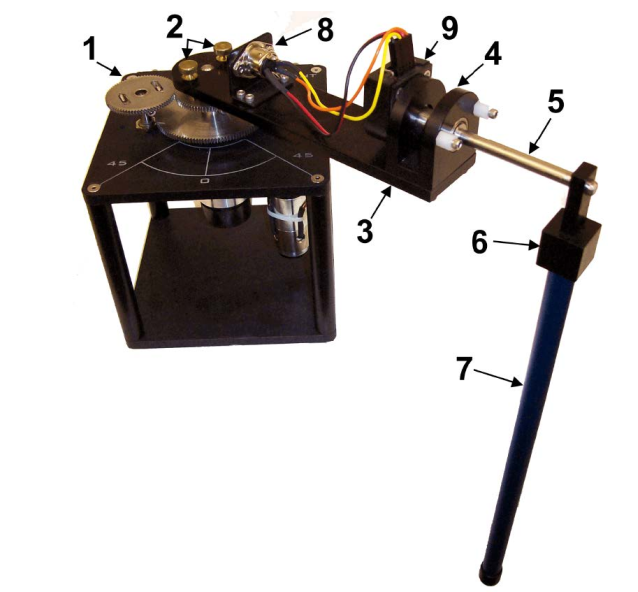
\includegraphics[scale=0.25]{pondule.png}
  \captionof{figure}{Composants du pendule}
  \label{fig1}
\end{minipage}%
\begin{minipage}{.5\textwidth}
	\begin{center}
		\begin{tabular}{|c|c|}
		\hline \rowcolor{rougecerise} $N^{0}$ & Composant\\
		\hline 1 & SRV02\\
		\hline 2 & Vis\\
		\hline 3 & Bras\\
		\hline 4 & Logement d’arbre\\
		\hline 5 & Arbre\\
		\hline 6 & Raccord\\
		\hline 7 & Pendule\\
		\hline 8 & Connecteur de l'encodeur\\
		\hline 9 & Encodeur\\
		\hline
		\end{tabular}
		\label{tab1}
		\captionof{table}{Nomenclature des composants de la maquette}
	\end{center}
\end{minipage}
\end{figure}

    %******************* MODÉLISATION **********
 \chapter{Modélisation}
 
 La Figure \ref{fig2} donne une représentation schématique du pendule. Le bras est relié au moteur, qui entraine la rotation du bras et donc du pendule. Il a une longueur \hspace{1mm} $L_{r}$\hspace{1mm} et un moment d’inertie \hspace{1mm} $J_{r}$. Nous noterons son angle\hspace{1mm} $\theta$.
 
 \paragraph{}
 Le pendule, quant à lui, est lixé au bout du bras. Il a une longueur \hspace{1mm} $L_{p}$. Son moment d’inertie au centre de masse est noté\hspace{1mm} $J_{p}$. On note l’angle que fait l’axe du pendule avec l’axe verticale\hspace{1mm} $\alpha$\hspace{1mm}(en radian).
 
 \paragraph{}
 Tous les calculs de la modélisation se feront en prenant pour origine, la position haute du pendule. Pour les descriptions et les valeurs numériques des constantes se reporter à la Table \ref{tab2}.
 
 \paragraph{}
 Les équations du mouvement, déterminées à l’aide de la mécanique Lagrangienne, sont données par les deux équations différentielles suivantes:\\
 
  \paragraph{}Equation 1:\\\\
$\bigg(m_{p}L_{r}^{2} + \frac{1}{4}m_{p}L_{p}^{2} - \frac{1}{4}m_{p}L_{p}^{2}cos(\alpha^{2}) + J_{r} \bigg)\ddot{\theta}- \bigg(\frac{1}{2}m_{p}L_{p}L_{r}\cos(\alpha) \bigg)\ddot{\alpha}+$\\  $\bigg(\frac{1}{2}m_{p}L_{p}^{2}\sin(\alpha)\cos(\alpha) \bigg)\dot{\theta}\dot{\alpha} + \bigg(\frac{1}{2}m_{p}L_{p}L_{r}\sin(\alpha) \bigg)\dot{\alpha}^{2}=\frac{\eta_{g}K_{g}\eta_{m}k_{t}(V_{m}- K_{g}k_{m}\dot{\theta})}{R_{m}}-B_{r}\dot{\theta}$ $\hspace{1mm}$ \\\\

    \paragraph{}Equation 2:\\\\
$-\frac{1}{2}m_{p}L_{p}L_{r}\cos(\alpha)\dot{\theta}+(J_{p}+\frac{1}{4}m_{p}L_{p}^{2})\ddot{\alpha}-\frac{1}{4}m_{p}L_{p}^{2}\cos(\alpha)\sin(\alpha)\dot{\theta}^{2}-\frac{1}{4}m_{p}L_{p}g\sin(\alpha)$\\\\$=-B_{p}\dot{\alpha}$   $\hspace{3mm}$ \\\\
 
\begin{center}
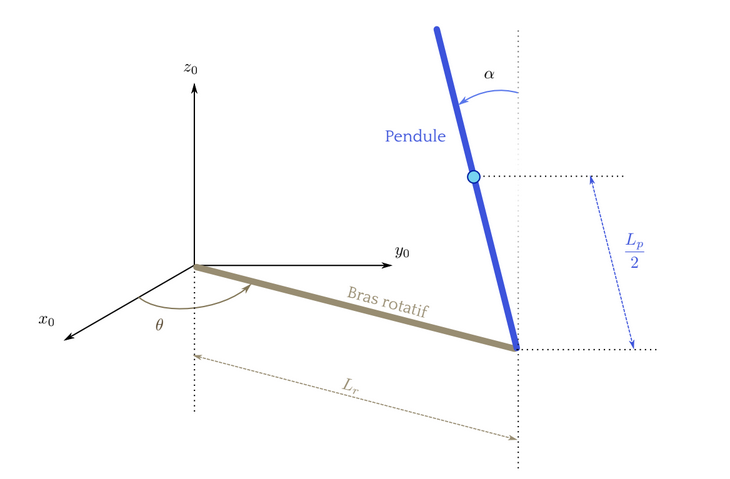
\includegraphics[scale=0.5]{shemadupendule.png}
\captionof{figure}{\textit{Schéma du pendule rotatif.}}
\label{fig2} 
\end{center}

\begin{center}
\begin{tabular}{|c|c|c|}
\hline \rowcolor{rougecerise} Symbole & Description &  Valeur  \\
\hline $B_{p}$  &  Coef de frottement visqueux du pendule  & $0.0024 kg/m^{2}$   \\
\hline $B_{r}$ & Coef de frottement visqueux du bras & $0.0024 kg/m^{2}$ \\
\hline $\eta_{g}$  &  Rendement du réducteur  & $0.9$  \\
\hline $\eta_{m}$  &  Rendement du moteur  & $0.69$  \\
\hline $K_{g}$  &  Rapport de vitesse  & $70$  \\
\hline $K_{m}$  &  Gain f.e.m  & $7.68\times10^{-3} V/(rad/s)$ \\
\hline $K_{t}$  &  Gain couple moteur/courant  & $7.68\times10^{-3} N.(m/A)$\\
\hline $J_{p}$ &  Moment d'inertie du pendule au ctr de masse & $0.0012 kg/m^{2}$ \\
\hline $J_{r}$  &  Moment d'inertie du bras au ctr de masse  & $9.98\times10^{-4} kg/m^{2}$ \\
\hline $L_{m}$  &   Inductance du moteur & $0.18 mH$\\
\hline $L_{p}$  &  longueur du pendule  & $0.337 m$ \\
\hline $L_{r}$  &  Inductance du bras, du pivot à l'extrémité   & $0.216 m$ \\
\hline $m_{p}$  &  Masse du pendule  & $0.127 kg$\\
\hline $m_{r}$  &   Masse du bras  & $0.257 kg$\\
\hline $R_{m}$  &   Résistance du moteur  & $2.60 \Omega$ \\
\hline $V_{m}$  &  Tension envoyé au moteur   &  A régler \\

\hline 
\end{tabular}
\captionof{table}{\textit{Liste des données spécifiques au système}}
\label{tab2}
\end{center} 

\section{Etude succincte du modèle non linéaire}

Dans un premier temps, nous allons étudier le modèle non linéaire représenté par les deux équations du mouvement Equation 1 et Equation 2.

 \subsection{Proposition des variables d'état}

 On choisit les variables :\hspace{1mm} $\theta$, $\dot{\theta}$  ,$\alpha$  et $\dot{\alpha}$ comme variables d'état.\\
 Soit on obtient le vecteur d'état suivant :\\
 \begin{center}
 $x = 
  \begin{bmatrix}
  \theta & \alpha & \dot{\theta} & \dot{\theta}
  \end{bmatrix}^{T}$ 
 \end{center}
 
 \subsection{Les points d'équilibre}
 
 En se servant de la Figure \ref{fig2} on va déterminer les points d'équilibre en fonction de la valeur de la tension $V_{m}$. Pour atteindre un point d'équilibre le système doit être immobile ou sans mouvement, ce qui implique que $\dot{\theta} = 0$ et $\dot{\alpha} = 0$, voyons ce que deviennent nos équations Lagrangiènnes vues précédemment:\\
  \begin{center}
Equation 1 :\hspace{1mm} $\frac{\eta_{g}K_{g}\eta_{m}k_{t}(V_{m}- K_{g}k_{m}\dot{\theta})}{R_{m}} = 0	\hspace{2cm}	(1)$ 
  \end{center}
  
  \begin{center}
Equation 2 :\hspace{1mm} $\frac{1}{4}m_{p}L_{p}g\sin(\alpha) = 0	\hspace{2.7cm}	(2)$ 
  \end{center}
   
De $(1)$ et de $(2)$ on remarque que pour avoir un équiblibre il faut que $V{m} = 0 \Rightarrow \theta = 0$ et que $sin(\alpha) = 0 \Rightarrow \alpha = k\pi, k \in Z .$ Le vecteur d'état deviens alors:\\



\begin{center}
 $x = 
  \begin{bmatrix}
  0 & k\pi & 0 & 0
  \end{bmatrix}^{T}$ 
 \end{center}
 
\textbf{Nota :} De la sorte on obtient une infinité de solutions ou de points d'équilibre stables $k  \hspace{1mm} pair $ et instables $k \hspace{1mm} impair.$

On pourra dire à la fin que les valeurs des points d'équilibre obtenus sont en accord avec le dispositif réel.

   \subsection{Simulation du dispositif non linéaire aux points d'équilibre}
 
  
\begin{center}
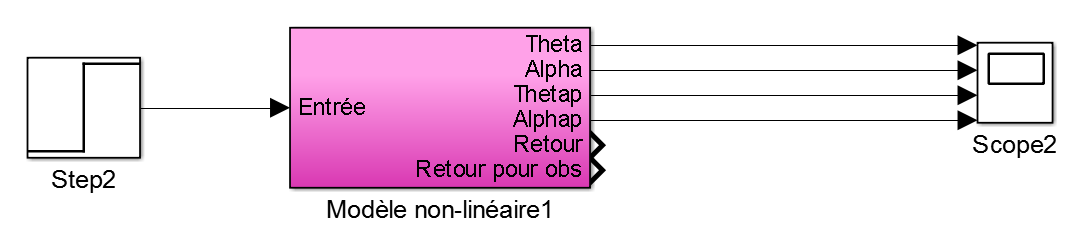
\includegraphics[scale=0.5]{modelenonlineairesimulink.png}
\captionof{figure}{\textit{Schema SIMULINK du modèle non linéaire}}
\label{fig3} 
\end{center} 
 
\begin{center}
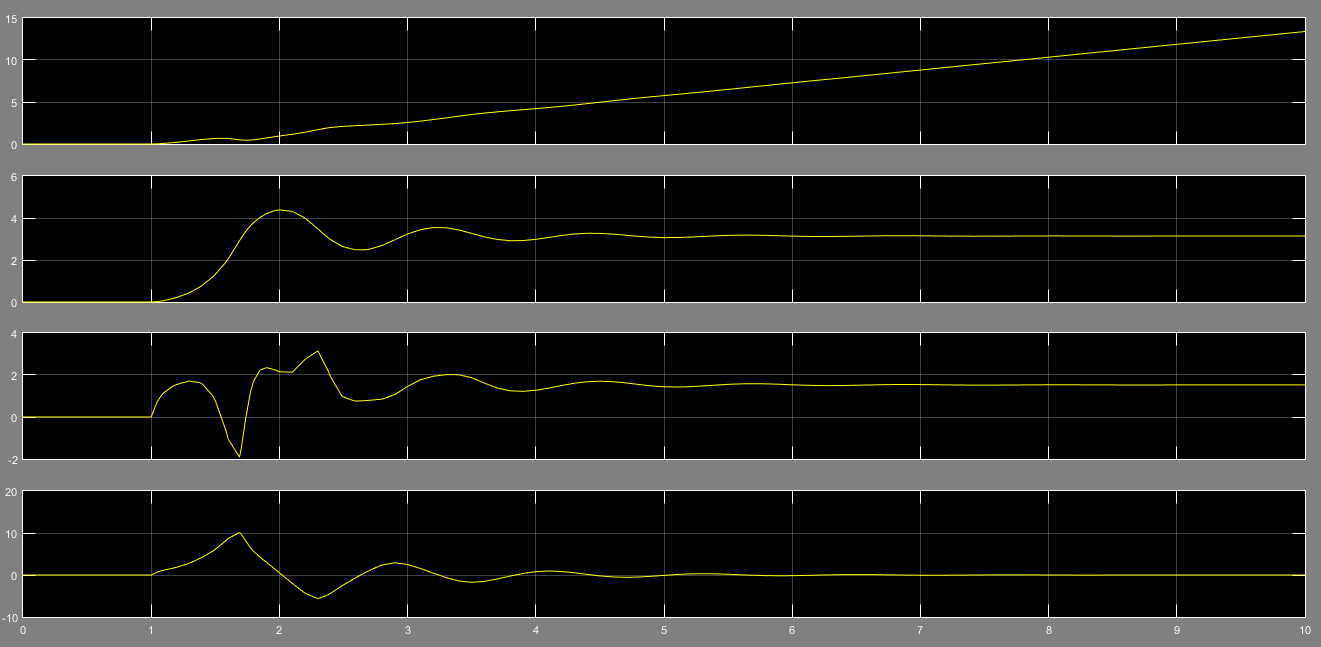
\includegraphics[scale=0.4]{modelenonlin1.PNG}
\captionof{figure}{\textit{Résultat SIMULINK du modèle non linéaire}}
\label{fig4} 
\end{center} 
 
 Le graphe montre que le modèle non linéaire converge vers un point d'équilibre instable car de la courbe 2:$\alpha = \pi$ et de la courbe 4: $\dot{\alpha}=0$, or  de la courbe 1: $\dot{\theta}$ diverge avec une vitesse constante $\dot{\theta} \simeq 2.$ De la sorte après un test sur le dispositif réel on a remarqué qu'au bout d'un moment on perd l'équilibre à cause des contreintes physiques que possède le pendule qu'on représentera comme un signal de bruit. 

\subsection{Simulation du dispositif non linéaire pour des conditions initiales}

Pour : $\alpha=+1$; $\theta=0$; $\dot{\alpha}=0$; $\dot{\theta} = 0$ \\
                                                   
\begin{center}
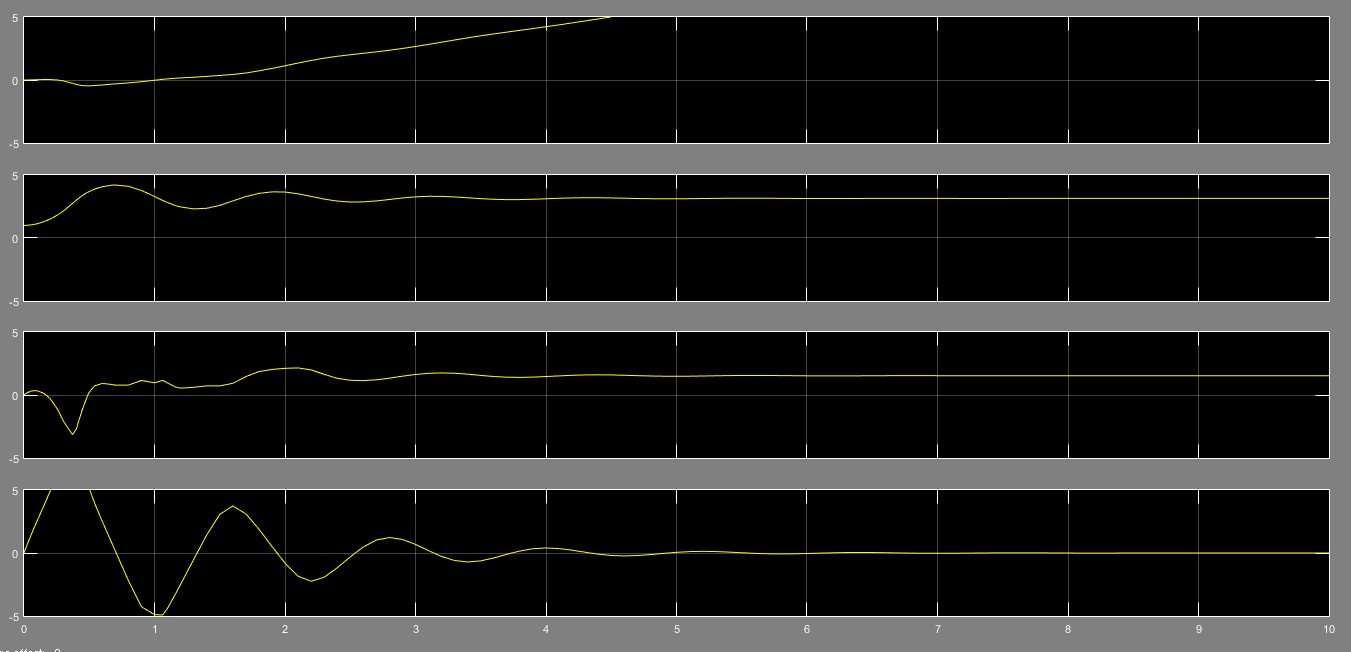
\includegraphics[scale=0.4]{alpha=+1.PNG}
\captionof{figure}{\textit{Résultat SIMULINK pour $\alpha=+1$.\\}}
\label{fig5} 
\end{center} 
Comme le cas précédent, on obtient un point d'équilibre en $ \alpha = \pi$ mais $\theta $ diverge toujours.  
 
Pour :
$\alpha=-1$; $\theta=0$; $\dot{\alpha}=0$; $\dot{\theta} = 0:$ \\
                                                   
\begin{center}
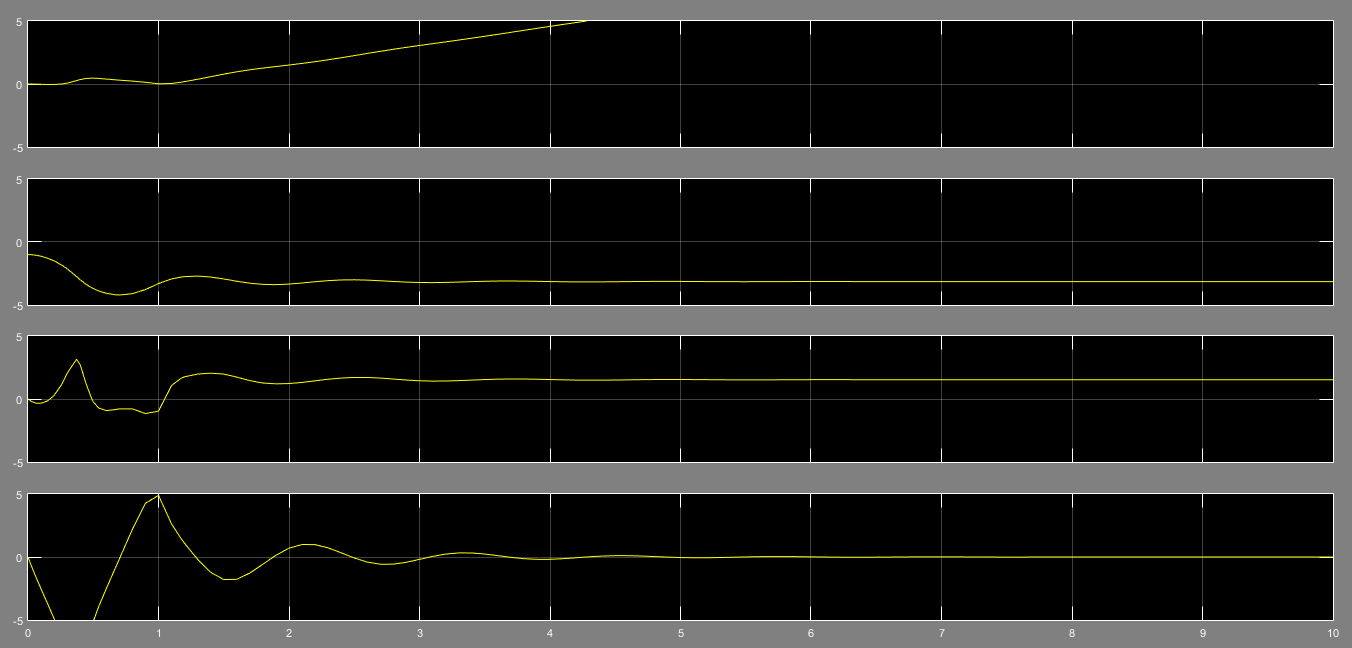
\includegraphics[scale=0.4]{alpha=-1.PNG}
\captionof{figure}{\textit{Résultat SIMULINK pour $\alpha=-1$.\\}}
\label{fig6} 
\end{center}
Cette fois ci, on obtient un point d'équilibre en $  \alpha = -\pi$. (Code Matlab voir\hyperref[section1.3]{Annexe A})\label{annexe1}.\\

\section{Linéarisation et obtention d'un modèle linéaire}

\subsection{Décomposition en série de Taylor}
 

La commande ss(A,B,C,D) sous Matlab a donné :\\
\begin{center}
 \[
   A_{up}=
  \left[ {\begin{array}{cccc}
   0 & 0 & 1 & 0 \\
    0 & 0 & 0 & 1 \\
     0 & 81.4033 & -28.8249 & -0.9319 \\
      0 & 122.0545 & -27.7372 & -1.3972 \\
  \end{array} } \right]
\]
 \[
   B_{up}=
  \left[ {\begin{array}{c}
   0 \\
   0 \\
   51.8323 \\
   49.8764 \\
  \end{array} } \right]
\]
 \[
   C_{up}=
  \left[ {\begin{array}{cccc}
   1 & 0 & 0 & 0 \\
    0 & 1 & 0 & 0 \\
  \end{array} } \right]
\]
\end{center}



 \chapter{Analyses temporelle et structurelle du modèle linéaire}
 
 A l'aide des fonctions de MATLAB on trouve que:\\
 	 \begin{itemize} [label=\ding{70},font=\small \color{black}]
 	 \item Le système n'est pas stable car un des pôles calculés : $[0 \hspace{2mm} -32.3450 \hspace{2mm} 7.3932 \hspace{2mm} -5.2702 ]$  possède une partie réelle positive.
 	 \item 
 	  Commandabilité:
 	 \begin{center}
 \[
Co =
  \left[ {\begin{array}{cccc}
   0 & 0.0001 & -0.0015 & 0.0499 \\
    0 & 0 & -0.0015 & 0.0509 \\
     0.0001 & -0.0015 & 0.0499 & -1.6077 \\
      0 & -0.0015 & 0.0509 & -1.6384 \\
  \end{array} } \right]
\]
     \end{center}
     $rang(Co) = 4 $ égale au nombre de pôles donc le système est commandable.
     \item 
     Observabilité:
 	 \begin{center}
 \[
  Obs =
  \left[ {\begin{array}{cccc}
   0.001 &  &  & 0 \\
    0 & 0.001 & 0 & 0 \\
     0 & 0 & 0.001 & 0 \\
     0 & 0 & 0 & 0.001 \\
      0 & 0.0814 & -0.0288 & -0.0009 \\
      0 & 0.1221 & -0.0277 & -0.0014 \\
      0 & -2.4602 & 0.8565 & 0.1096 \\
      0 & -2.4284 & 0.8383 & 0.1499 \\     
  \end{array} } \right]
\]
     \end{center}
     $rang(Obs) = 4 $ égale au nombre de pôles donc le système est observable.
 	 \end{itemize}\hyperref[section1.11]{(voir Annexe B)}\label{annexe11}
  
 \chapter{Régulation d'un modèle linéarisé}
On a choisit de prendre $p=
  \begin{bmatrix}
  -108&-0.3&-4.3+2.2i&-4.3-2.2i
  \end{bmatrix}^{T}$ comme valeurs propres car elle ont toutes une partie réelle négative dans le but stabiliser le système.
    
    \section{Simuler la réponse aux conditions initiales sur le modèle linéaire}          
       
\begin{center}
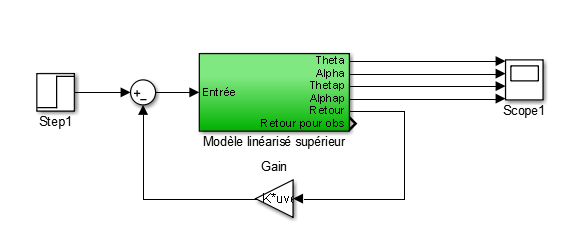
\includegraphics[scale=0.6]{oon.png}
\captionof{figure}{\textit{Schema SIMULINK du retour d'état sur le modèle linéaire}}
\label{fig7}
\end{center}

En utilisant le commande $acker$ on obtient les pôles désirés de la sorte : $ K_{up} = [-4.4472 \hspace{3mm}36.9886 \hspace{3mm} -3.3994 \hspace{3mm} 5.3447] $\hyperref[section1.111]{(voir Annexe C)}\label{annexe111}\\
On remplace ces valeurs dans le gain verctoriel sur SIMULINK et on obtient : 
  
\begin{center}
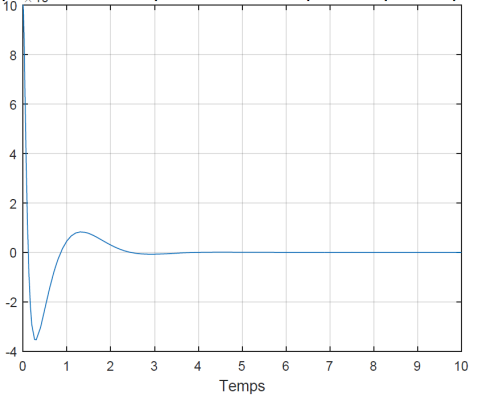
\includegraphics[scale=0.7]{figue2.png}
  \captionof{figure}{Résultat SIMULINK avec retour d'état courbe de $\theta $}
\label{fig8}
\end{center}

\begin{center}
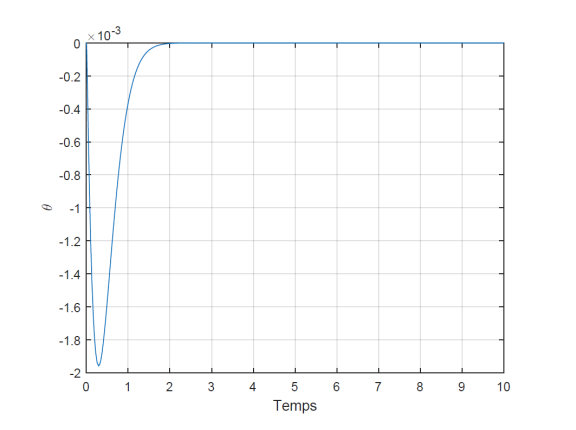
\includegraphics[scale=0.7]{figue1.png}
  \captionof{figure}{Résultat SIMULINK avec retour d'état  courbe de $\alpha $}
\label{fig9}
\end{center}
On remarque que la courbe $\theta$ et celle de $\alpha$ convergent vers une valeur finie, donc le système en boucle fermée est normalement stable.\\

\textbf{Nota : } Après implémentation de la loi de commande sur le dispositif réel et après expérience on remarque que l'angle $\theta$ n'est pas fixe et donc notre commande n'est pas assez robuste.
  


     
      % *********************** Conclusion *****************  








\begin{appendices}
\chapter*{Annexe A}
	\addcontentsline{toc}{chapter}{Annexe A}		
		Code Matlab, partie initialisations \hyperref[annexe1]{(Section 1.3)}\label{section1.3}
		\begin{lstlisting}
			%Reglage de Te et de l'initialisation
    			Te=0.02;
    			Theta_init=0;
    			Alpha_init_nl=-1; %ou=1 %Origine en haut
    			Alpha_init_sup=0; %Origine en haut
    			Alpha_init_inf=0; %Origine en bas    			
		\end{lstlisting}
		%\hyperref[sec:hello]{Retour vers Section 1.1}
		.\\\\\\
		Code Matlab chapitre 2 \hyperref[annexe11]{(Retour vers Chapitre 2)}\label{section1.11}
		%\hyperref[section1.11]{voir Annexe 1}\label{annexe11}.
		\begin{lstlisting}
			%Appel des fichiers
			Espace_etat_ABCD; % A COMPLETER genere {A,B,C,D}{up,int,down}
			systeme_haut = ss(Aup,Bup,Cup,Dup)
			poles = eig(Aup) %1ere question
			com = ctrb(Aup,Bup) %2eme question
			rangcom = rank(com)%2eme question
			obs = obsv(Aup,Cup)%3eme question
			rangobs = rank(obs)%3eme question		    			
		\end{lstlisting}
		.\\\\\\
		Code Matlab pour trouver K\hyperref[annexe111]{(Retour vers chapitre 4)}\label{section1.111}
		\begin{lstlisting}
			%%Chapitre 4
			K =  acker(Aup,Bup,[-108 -0.3 -4.3+2.2*i -4.3-2.2*i])  			
		\end{lstlisting}
				
\end{appendices}





%Bibliographie 
%\bibliographystyle{alpha}
%\bibliography{biblio}




\end{document}





